\documentclass[12pt]{amsart}
%\usepackage{algpseudocode}
\usepackage{algorithm}
\usepackage[noend]{algpseudocode}
\usepackage{amsmath}
\usepackage{amsfonts}
\usepackage{amssymb}
\usepackage[utf8]{inputenc}
\usepackage{listings}
\usepackage[pdftex]{hyperref}
\usepackage{caption}
\usepackage{subcaption}
\usepackage{geometry}

\geometry{
 letterpaper,
 total={8.5in,11in},
left=25mm,
right=25mm, 
top=20mm,
bottom=20mm,
}
 \usepackage{setspace}
\doublespace 
\usepackage[document]{ragged2e}

\usepackage{helvet}
\renewcommand{\familydefault}{\sfdefault}

\usepackage{blindtext}

\usepackage[spanish]{babel}

\usepackage{graphicx}
\usepackage{epsfig}


%-----------------------------------------------------------------------------------
% Configuración
%-----------------------------------------------------------------------------------
\hypersetup{colorlinks,%
	    citecolor=black,%
	    filecolor=black,%
	    linkcolor=black,%
	    urlcolor=blue}

%-----------------------------------------------------------------------------------
% Algorithm
%-----------------------------------------------------------------------------------

%\usepackage[ruled,vlined,lined,linesnumbered,portuguese]{algorithm2e} %permite escribir pseudocodigo
%  \setcounter{secnumdepth}{3}
%  \setcounter{tocdepth}{3}
%  \numberwithin{equation}{chapter}
%===================================================================================


\begin{document}

\begin{center}
    {\large Universidad de La Habana}  \\ 
    \vskip 0.1cm
    {\LARGE \textbf{T\'ITULO DEL TRABAJO}} \\
    \vskip 2cm
    {\Large Autores:}\\ 
    \vspace{0.5cm} 
            {\Large\textbf{Daniela Rodr\'iguez}} \\
    		{\normalsize\textit{daniela.rodriguez@estudiantes.matcom.uh.cu}}\\
    		MATCOM\\
			\smallskip
    		{\Large\textbf{Carlos Carret}} \\
    		{\normalsize\textit{carlos.carret@estudiantes.matcom.uh.cu}}\\
			MATCOM\\
			\smallskip
 			{\Large\textbf{Belsai Arango}} \\
 			{\normalsize\textit{belsai.arango@estudiantes.matcom.uh.cu}}\\
 			MATCOM \\
 \smallskip
 \smallskip
    {\Large Tutor:\\ 
    \vspace{0.05cm} 
    		\textbf{Reinaldo Rodr\'iguez Ramos}} \\ 
    		\textit{reinaldo@matcom.uh.cu}\\
    		MATCOM \\   
  \vskip 1.5cm
  
  \Large \textbf{Resumen}:
  Debido a que la vida humana se encuentra en constante peligro por enfermedades como el c\'ancer una vez que se encuentran en etapas finales, se realiza un estudio para crear representaciones matem\'aticas y herramientas computacionales para el estudio de sus comportamientos en etapa vascular y avascular y obtener un acercamiento mediante estas a la realidad. Para esto se confecciona un modelo estoc\'astico cuya especializaci\'on va orientada hacia el c\'ancer en el tejido epitelial, adem\'as simula y muestra el crecimiento tumoral en 3D.
    
  \end{center}
  
\newpage
\section{Introducci\'on}
El c\'ancer de mama representa un peligro para la vida humana, m\'as a\'un si se encuentra en fases avanzadas de su desarrollo, por eso esta investigaci\'on tiene como objetivo producir representaciones matem\'aticas y herramientas computacionales que permiten estudiar dichos comportamientos. Para obtener una simulaci\'on y un mayor acercamiento a la realidad del comportamiento de un tumor en su etapa vascular y avascular se confecciona el presente modelo estoc\'astico. En este se analiza cada etapa, as\'i como las variaciones de los par\'ametros y partes que intervienen en las mismas, bas\'andose en el proceso de acumulaci\'on de mutaciones. La especializaci\'on del c\'ancer en el que se profundiza es el carcinoma, es decir el desarrollo del c\'ancer en el tejido epitelial, teniendo
en cuenta el ciclo biol\'ogico del organismo, las interacciones y transiciones entre los diferentes tipos de c\'elulas cancer\'igenas, normales e inmunes, tambi\'en se repoduce el crecimiento tumoral hacia las distintas capas de tejidos del p\'ancreas, la invasi\'on del estroma del \'organo y el proceso de migraci\'on de las c\'elulas a trav\'es del tejido. Por \'ultimo mostrar de forma gr\'afica el proceso de crecimiento del tumor en 3D.

\newpage
\section{\bf{Desarrollo}}

\section{\bf{Definici\'on del modelo}}
Para la creaci\'on del modelo del aut\'omata, se hacen algunas consideraciones a partir de la propia evoluci\'on del tumor segun referencias brindadas en\cite{1}.


\subsection{Hip\'otesis del modelo}
\begin{enumerate}

\item {{\it C\'elulas inmunitarias: }} Consideramos a diferentes c\'elulas inmunitarias, como B, T, APC, PLB,\footnote{{\it C\'elula B:} se le llaman linfocitos B que se forman a partir de las c\'elulas madre en la m\'edula \'osea. Estas c\'elulas se activan y maduran a c\'elulas plasm\'aticas, las cuales producen y liberan anticuerpos que con sus mol\'eculas efectoras.\\ {\it C\'elula T:} es otro tipo de linfocito que se desarrolla a partir de c\'elulas progenitoras de la m\'edula \'osea que viajan hasta el timo.\\ {\it C\'elula APC:} c\'elulas presentadoras de ant\'igenos.\\ {\it C\'elula LBP:} prote\'ina de uni\'on a lipopolisac\'arido. El lipopolisac\'arido desempe\~na una importante funci\'on en la activaci\'on del sistema inmune al constituir el ant\'igeno superficial m\'as importante de este tipo de bacterias} en el sistema de inmunidad tumoral como componente \'unico celular "c\'elulas de inmunidad".
\item {\it Entidades del modelo:} Las entidades biol\'ogicas presentes en el modelo se componen \'unicamente de los tipos de c\'elulas definidos en el conjunto de estados del aut\'omata celular, el cual est\'a compuesto por tres poblaciones celulares: c\'elulas normales, c\'elulas tumorales y c\'elulas de inmunidad.
\item {\it Interacciones entre las c\'elulas:} Las interacciones entre las distintas c\'elulas del modelo se componen solamente por las reglas definidas en la funci\'on de transici\'on del aut\'omata. Hay tipos de acciones celular que son respecto al movimiento celular: proliferaci\'on celular y dos tipos de interacciones en el sistema del modelo, entre las c\'elulas normales y las c\'elulas tumorales, y entre las c\'elulas tumorales y c\'elulas inmunitarias.

\item {\it Progresi\'on idealizada del desarrollo tumoral:} Se asume que el desarrollo tumoral sigue una progresi\'on idealizada dividida en las etapas avascular y vascular, donde el comportamiento macrosc\'opico del tumor est\'a definido por las mutaciones que expresan las c\'elulas cancer\'igenas.

\item {\it Mutaciones de las c\'elulas cancer\'igenas:} Se asume que la acumulaci\'on de mutaciones en la c\'elula cancer\'igena se define como un proceso secuencial y sigue un orden establecido, es decir, durante la etapa avascular se expresan las mutaciones relacionadas con el ciclo celular y la proliferaci\'on tumoral, y durante la etapa vascular se expresan las mutaciones relacionadas con la angiog\'enesis y met\'astasis, en adici\'on a las anteriores.

\item {\it Invarianza de las c\'elulas normales:} Se asume que la poblaci\'on de c\'elulas normales del organismo es est\'atica e invariante durante el transcurso del tiempo, es decir, no incurren en los procesos de divisi\'on ni muerte celular.

\item {\it Homogeneidad de las c\'elulas cancer\'igenas:} Se asume que la poblaci\'on de c\'elulas cancer\'igenas que conforma la masa de un tumor es homog\'enea, es decir, no existen subtipos con mutaciones distintas o que est\'en en distintas etapas del ciclo celular.

\item {\it Suficiencia de nutrientes:} Se asume que el suministro de nutrientes y ox\'igeno es constante y suficiente para que todo tumor representado en el aut\'omata celular se desarrolle adecuadamente.

\item{\it Desarrollo tumoral en funci\'on de la poblaci\'on:} Se asume que el avance de un tumor a trav\'es de las distintas etapas de su desarrollo depende \'unicamente de su poblaci\'on celular, descrita por la ecuaci\'on de Verhulst de crecimiento log\'istico.

\item  {\it Adhesi\'on celular:} Se asume que la adhesi\'on de las c\'elulas tumorales se mantiene en todo momento salvo en los desprendimientos de c\'elulas migratorias como parte de la cascada metast\'asica.

\item {\it V\'ias de la met\'astasis:} Se consideran solamente la diseminaci\'on hem\'atica y linf\'atica como v\'ias de la met\'astasis.

\item {\it Representaci\'on del tejido:} Se asume que un tejido puede ser representado mediante una red de mundo peque\~no, generada a partir del modelo Watts-Strogatz. % donde las coordenadas de los v\'ertices poseen dos componentes $x, y \in \mathbb{N}$ que constituyen la localizaci\'on de la c\'elula en el plano correspondiente con un corte de dicho tejido.

\end{enumerate}
\newpage
\subsection{Modelo Watts-Strogatz}

Se adapta  el modelo de Watts-Strogatz  \footnote{{\it Watts-Strogatz:} es un algoritmo para redes de mundo peque\~no que establece una red inicial unidimensional con N nodos, estos nodos se pueden disponer en forma de anillo de tal forma que cada uno de los v\'ertices (o nodos) se una con 2k vecinos. La probabilidad de conectar un nodo con otro cualquiera es de p. Para un grafo con p=0 se puede ver que la conectividad es la misma y de valor 2k. por otro lado un valor no nulo de p introduce desorden en la red de tal forma que la conectividad no es uniforme, manteniendo todavía de media un valor de 2k.\\{\it Red de Mundo Pequeño: }es un tipo de grafo para el que la mayoría de los nodos no son vecinos entre sí, y sin embargo la mayoría de los nodos pueden ser alcanzados desde cualquier nodo origen a través de un número relativamente corto de saltos entre ellos.\\} implementado en \cite{1}, para utilizarlo en un plano tridimensional por lo que se realizan algunas modificaciones tales como: 
\begin{enumerate}
\item A la distancia euclideana se le agregada una nueva componente al llevar de R2 a R3 por lo que la f\'ormamula quedar\'ia :  $d_E(v,w)= \sqrt{ (v_x-w_x)^2 + (v_y-w_y)^2 + (v_z-w_z)^2}  $\\
\item Implementaci\'on del Modelo Watts-Strogatz en 3D.\\
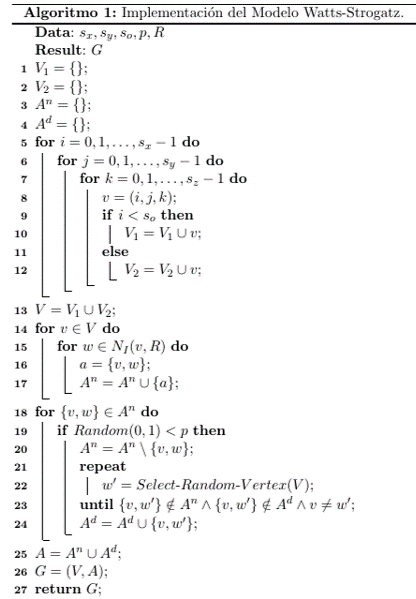
\includegraphics[scale=0.7]{img/Picture1.png}
\end{enumerate}

\newpage
\subsection{Conjunto de estados}
El tejido epitelial recubre toda superficie del cuerpo humano que tiene contacto con el exterior, e.g. \'organos huecos, como el est\'omago y pulmones, o estructuras tubulares, como los bronquios y arterias. En los carcinomas es com\'un que la masa tumoral brote fuera del epitelio, evadiendo los controles de homeostasis del tejido y volvi\'endose una lesi\'on. La manifestaci\'on fuera del epitelio constituye un marcador visible del desarrollo neopl\'asico, por lo que la luz de un \'organo o lumen debe ser representada.

Se definen los siguientes estados:

{\it C\'elulas normales en el aut\'omata:}  
\begin{itemize}
\item s($v$, $n$) = 0: El v\'ertice $v$ posee el estado correspondiente con el espacio vac\'io o lumen en el instante de tiempo $n$, y representa las cavidades huecas de los \'organos y conductos.
\item s($v$, $n$) = 1: El v\'ertice $v$ representa una c\'elula del epitelio en el instante de tiempo $n$, y corresponde con el tejido donde se origina el carcinoma.
\item s($v$, $n$) = 2: El v\'ertice $v$ posee el estado correspondiente con el estroma en el instante de tiempo $n$, y representa el conjunto de tejidos de sost\'en del \'organo.
\end{itemize}

{\it C\'elulas inmunes}: 
\begin{itemize}
\item s($v$, $n$) = 3: El v\'ertice $v$ posee el estado correspondiente con el espacio vac\'io o lumen en el instante de tiempo n, y representa las cavidades huecas de los \'organos y conductos.
\item s($v$, $n$) = 4: El v\'ertice $v$ representa una c\'elula del epitelio en el instante de tiempo $n$, y corresponde con el tejido donde se origina el carcinoma.
\item s($v$, $n$) = 5: El v\'ertice $v$ posee el estado correspondiente con el estroma en el instante de tiempo $n$, y representa el conjunto de tejidos de sost\'en del \'organo.
\item s($v$, $n$) = 6: El v\'ertice $v$ representa una c\'elula inmune en el sistema circulatorio en el instante de tiempo $n$.
\item s($v$, $n$) = 7: El v\'ertice $v$ representa una c\'elula inmune en el \'organo secundario, es decir donde se hizo met\'astasis.
\end{itemize}
{\it C\'elulas cancer\'igenas:} 
\begin{itemize}
\item s($v$, $n$) = 8: El v\'ertice $v$ representa una c\'elula tumoral en el instante de tiempo $n$, y constituyen la masa neopl\'asica.
\item s($v$, $n$) = 9: El v\'ertice $v$ representa una c\'elula migratoria en el instante de tiempo $n$, es decir, poseen las mutaciones necesarias para efectuar la cascada metast\'asica.
\item s($v$, $n$) = 10: El v\'ertice $v$ representa una c\'elula micrometast\'asica en el instante de tiempo $n$, es decir, efectuaron la cascada metast\'asica satisfactoriamente y est\'an colonizando la nueva localizaci\'on, pero pueden ser destruidas por el sistema inmunitario o fallar en dicha colonizaci\'on.

\end{itemize}



\subsection{Funci\'on de transici\'on}
La funci\'on de transici\'on general utilizada en el aut\'omata estoc\'astico est\'a definida localmente. Las reglas aplicadas a las c\'elulas est\'an condicionadas por una variable aleatoria que determina la probabilidad del pr\'oximo estado de una c\'elula a partir de su estado actual y de los estados que posean las c\'elulas vecinas a ella.
\label{subsec:funcion de transicion}
\subsubsection{Reglas de la conservaci\'on del estado de c\'elulas normales, inmunes y tumorales}

Las c\'elulas normales se mantienen est\'aticamente y su estado no var\'ia a menos que exista la presencia de c\'elulas cancer\'igenas o de inmunidad en su vecindad.\\
Las c\'elulas de inmunidad solo cambian a una posici\'on espec\'ifica cuando existe la presencia de c\'elulas cancer\'igenas en su vecindad.\\
Las c\'elulas inmunitarias se mueven libremente hacia las c\'elulas normales.
Al comienzo de cada instante de tiempo las c\'elulas de inmunidad seleccionan una de las posibles vecinas inmediatas para desplazarse. Si la probabilidad de moverse hacia un vecino $w$ es menor que un valor $th$, la c\'elula de inmunidad mantiene su posici\'on inicial. Formulamos la regla de la siguiente forma:\\
%$L(t+T) \xrightarrow{P_{w}} w \xrightarrow{P_m} \displaystyle \left\{ {L(t) \hspace{1cm} P_w<th \atop L(t + 1) \hspace{.5cm} P_w \geq th } \right\},$\\
$L(t+T) \xrightarrow{P_{w}} w  \displaystyle \left\{ {L(t) \hspace{1cm} P_w<th \atop L(t + 1) \hspace{.5cm} P_w \geq th } \right\},$\\

donde:\\
 $L(t):$ es la posici\'on de la celda;  $th:$ es el valor del umbral de movimiento;
 $P_{w}:$ es la probabilidad de moverse hacia el vecino $w$. 
 %$P_m:$ es la probabilidad de moverse o no hacia la posici\'on correspondiente.\\


\subsubsection{Regla de Inmunoreacci\'on}
Cuando las c\'elulas tumorales aparecen en la vecindad inmediata de las c\'elulas de inmunidad, las c\'elulas inmunes invaden la posici\'on de la c\'elula tumoral. En estos momentos decimos que ocurre inmunoreacci\'on. Luego ambas c\'elulas comienzan a combatir y se pueden dar 3 situaciones como resultado:
\begin{itemize}
\item La c\'elula de inmunidad mata a la c\'elula tumoral y la c\'elula se recupera, quedando en esta posici\'on una c\'elula normal.
\item La c\'elula tumoral vence a la c\'elula inmune y contin\'ua infectando y proliferando las c\'elulas normales.
\item Ambas c\'elulas no son lo suficientemente fuertes para derrotar a su rival, entonces la posici\'on donde estaba la c\'elula tumoral pasa a un estado intermedio, el cual puede cambiar al estado de c\'elula normal o tumoral, en dependencia de la cantidad de c\'elulas inmunes ,normales y tumorales que se encuentren en su vecindad inmediata.
\end{itemize}
$$Tc + Ic \xrightarrow{P_{I}} \displaystyle \left\{ \begin{tabular}{r l}
$Nc$ & $P_{I} < Th$ \\
$Mc$ & $P_{I} = Th$ \\
$Tc$ & $P_{I} > Th$ \\
\end{tabular} \right\} $$

 $Ic$: c\'elula inmune; $Nc$: c\'elula normal;  $Mc$: c\'elula en etapa intermedia;  $Tc$: c\'elula tumoral; $Th$: valor del umbral de inmunoreacci\'on; $p$: probabilidad de inmunoreacci\'on.

\subsubsection{Regla del Estado Intermedio}
Cuando las c\'elulas de inmunidad y las c\'elulas tumorales interact\'uan entre s\'i, uno de los resultados es que aparecen c\'elulas en etapa intermedia en el sistema. Si la suma de las c\'elulas normales y c\'elulas inmunes es mas que el 60\% de las c\'elulas vecinas, entonces las c\'elulas en un estado intermedio pasan a convertirse a c\'elulas normales. En caso de tener m\'as del 30\% de sus c\'elulas vecinas siendo tumorales, la c\'elula en estado intermedio pasar\'ia se convertir\'ia en una c\'elula tumoral.\\
$$Tc + Ic \xrightarrow \displaystyle \left\{ 
\begin{tabular}{r l}
$Nc$ & $Nc + Ic > 60\%$ \\
$Tc$ & $Tc > 30\%$ \\
\end{tabular} \right\} $$

\newpage
\section{\bf{Simulaci\'on del modelo en 3D}}
\subsection{Par\'ametros utilizados en la simulaci\'on }
A continuaci\'on se muestra una serie de tablas que contienen los par\'ametros que fueron insertados al modelo %y constantes utilizados en el modelo.\\

\begin{figure}[h!]%
		\begin{center}
			\begin{tabular}{|c|c|c|} \hline
			Par\'ametro & Descripci\'on  	                       & Valor 	\\ \hline
			%$P_m$       & Probabilidad de moverse o no &$0 \leq P_m  < 1  $			\\ \hline
			$P_w$       & Probabilidad de movimiento hacia el vecino w&$0 \leq P_w  < 1  $			\\ \hline
			$P_I$ 	    & Probabilidad de inmunoreacci\'on         &$0 \leq P_I  < 1  $			\\ \hline
			$Th$		& Valor del umbral de inmunoreacci\'on     & 0.43			\\ \hline
			$th$		& Valor del umbral de movimiento           & 0.5 			\\ \hline
			\end{tabular}
		\caption{Par\'ametros utilizados en la inmunoreacci\'on. \label{fig:inmune_param}\ref{subsec:funcion de transicion}}
		\end{center}
		\end{figure}

\begin{figure}[h!]%
		\begin{center}
			\begin{tabular}{|c|c|c|} \hline
			Par\'ametro & Descripci\'on  	                       & Escala 	\\ \hline
			$s_x$ & Dimensi\'on del espacio con respecto a las x    & $0 \leq x < s_x$      			\\ \hline
            $s_y$ & Dimensi\'on del espacio con respecto a las y    &	$0 \leq y < s_y$\\ \hline
            $s_z$ & Dimensi\'on del espacio con respecto a las z    &	$0 \leq z < s_z$\\ \hline
			$s_o$		      & Valor que marca la divisi\'on de la red entre los \'organos  & $0 \leq s_o < s_x $    \\ \hline
%			$p$		          & Probabilidad de reconexi\'on del modelo Watts-Strogatz.&  			\\ \hline
			\end{tabular}
		\caption{Par\'ametros de la construcci\'on de la red utilizados por el modelo Watts-Strogatz. \label{table-network-params}}
		\end{center}
		\end{figure}

%\begin{figure}[!ht]
%\begin{center}
%\scalebox{0.9}{\begin{tabular}{|p{2cm}|p{14.5cm}|} \hline
%\emph{Par\'ametro} & \emph{Descripci\'on} \\\hline
%\multicolumn{1}{|c|}{$P_0^a$, $P_0^v$} & Poblaciones iniciales de las etapas avascular y vascular respectivamente. \\\hline
%\multicolumn{1}{|c|}{$r_a$, $r_v$} & Ritmos de proliferaci\'on de las etapas avascular y vascular respectivamente. \\\hline
%\multicolumn{1}{|c|}{$K_a$, $K_v$} & Capacidad de carga de las etapas avascular y vascular respectivamente. \\\hline
%\multicolumn{1}{|c|}{$\Delta t$} & Tiempo transcurrido entre los instantes de tiempo $n$ y $n+1$. \\\hline
%\multicolumn{1}{|c|}{$n_a$} & Tiempo que permanece un tumor en etapa avascular. \\\hline
%\end{tabular}}
%\caption{Par\'ametros correspondientes con la ley de crecimiento log\'istico. \label{table-logistic-params}}
%\end{center}
%\end{figure}

%\begin{figure}[!ht]
%\begin{center}
%\scalebox{0.9}{\begin{tabular}{|p{2cm}|p{14.5cm}|} \hline
%\emph{Par\'ametro} & \emph{Descripci\'on} \\\hline
%\multicolumn{1}{|c|}{$o_l$} & Cantidad de capas del lumen.\\\hline
%\multicolumn{1}{|c|}{$o_e$} & Cantidad de capas del epitelio. \\\hline
%\multicolumn{1}{|c|}{$o_s$} & Cantidad de capas del estroma. Se determina como la cantidad de capas restantes en la red una vez que se disponen el lumen y el epitelio, es decir $o_s=s_y - (o_l + o_e)$.\\\hline
%\multicolumn{1}{|c|}{$v_x^t$, $v_y^t$,$v_z^t$} & Coordenadas de la c\'elula cancer\'igena central del tumor inicial. La disposici\'on inicial del tumor se determina a partir de las coordenadas de esta c\'elula central. Se asume que la coordenada $v_y^t$ pertenece al siguiente rango de valores: $v_y^t \in [o_l, o_l + o_e]$, y generalmente $v_x^t = s_x/4$. \\\hline
%\end{tabular}}
%\caption{Par\'ametros utilizados en la asignaci\'on de los estados iniciales a las c\'elulas del aut\'omata.\label{table-states-params-1}}
%\end{center}
%\end{figure}

\begin{figure}[!ht]
\begin{center}
\scalebox{0.9}{\begin{tabular}{|p{2cm}|p{14.5cm}|} \hline
\emph{Par\'ametro} & \emph{Descripci\'on} \\\hline
%\multicolumn{1}{|c|}{$o_e$} & Cantidad de capas del epitelio.\\\hline
%\multicolumn{1}{|c|}{$o_d$} & Coordenada de la l\'inea central del ducto mamario. Se extiende por los puntos $(v_x,o_d)$ para todo $v \in V(G)$.\\\hline
%\multicolumn{1}{|c|}{$R^d$} & Radio del ducto mamario representado. Se itera por los v\'ertices $v \in V(G)$ de coordenadas $v = (v_x,v_y)$ y seg\'un la distancia euclideana~(Def. \ref{def-euclidean-distance}) entre dicho v\'ertice y su correspondiente en la l\'inea central del ducto mamario $v^d = (v_x,o_d)$ se le asigna uno de los estados correspondientes con c\'elulas normales: si $d_E(v,v^d) > R^d + o_e$ se asigna el estado $2$ correspondiente con el estroma; si $d_E(v,v^d) \in [R^d, R^d + o_e]$ se asigna el estado $1$ correspondiente con el epitelio; y si $d_E(v,v^d) < R^d$ se asigna el estado $0$ correspondiente con el lumen.\\\hline
\multicolumn{1}{|c|}{$v_x^t$, $v_y^t$,$v_z^t$} & Coordenadas de la c\'elula cancer\'igena central del tumor inicial. La disposici\'on inicial del tumor se determina a partir de las coordenadas de esta c\'elula central. Se asume que la coordenada $v_y^t$ pertenece a los siguientes rangos de valores: $v_y^t \in [o_d + R^d, o_d + (R^d + o_e)]$ y $v_y^t \in [ o_d - (R^d + o_e), o_d - R^d]$, y generalmente $v_x^t = s_x/4$. \\\hline
\end{tabular}}
\caption{Par\'ametros utilizados en el procedimiento de actualizaci\'on y en el ajuste de las reglas del aut\'omata celular.\label{table-states-params-2}}
\end{center}
\end{figure}

%\begin{figure}[!ht]
%\begin{center}
%\scalebox{0.9}{\begin{tabular}{|p{2cm}|p{14.5cm}|} \hline
%\emph{Par\'ametro} & \emph{Descripci\'on} \\\hline
%\multicolumn{1}{|c|}{$\mu_{mig}$} & Cantidad de movimientos tentativos que la c\'elula migratoria puede llevar a cabo en un instante de tiempo.\\\hline
%\multicolumn{1}{|c|}{$\mu_{max}$} & Distancia m\'axima de migraci\'on.\\\hline
%\multicolumn{1}{|c|}{$\xi_{sc}$} & Probabilidad de supervivencia de una c\'elula migratoria durante el transporte en el sistema circulatorio.\\\hline
%\multicolumn{1}{|c|}{$\xi_{mic0}$,$\xi_{mic1}$} & Probabilidad de supervivencia de una micromet\'astasis.\\\hline
%\multicolumn{1}{|c|}{$\psi_{mic0}$,$\psi_{mic1}$} & Probabilidad de colonizaci\'on de una micromet\'astasis.\\\hline
%\multicolumn{1}{|c|}{$\eta_{mig}$} & Par\'ametro de ajuste de la probabilidad de transici\'on relacionada con la aparici\'on de c\'elulas migratorias.\\%%\hline
%\multicolumn{1}{|c|}{$K_{mig}$} & Par\'ametro de ajuste de la probabilidad de transici\'on relacionada con la aparici\'on de c\'elulas migratorias.\\\hline
%\multicolumn{1}{|c|}{$\eta_{mig}'$} & Par\'ametro de ajuste de la probabilidad de transici\'on relacionada con la muerte de c\'elulas migratorias durante su desplazamiento.\\\hline
%\end{tabular}}
%\caption{Par\'ametros utilizados en el procedimiento de actualizaci\'on y en el ajuste de las reglas del aut\'omata celular.\label{table-model-params}}
%\end{center}
%\end{figure}

%{\color{red} Falta la sangre, musculos, solo esta el esqueleto. Donde se ve la insercion de las tablas en el modelo propuesto por ustedes. Es decir, los resultados numericos.}\\

Los par\'ametros $s_z$ y $v_z^t$ fueron agregados como consecuencia de la conversi\'on del modelo del plano 2D a 3D. Los par\'ametros de la tabla~\ref{table-network-params} fueron utilizados para la representaci\'on del grafo a un plano en 3D a parir de una matriz, estos delimitan los valores m\'aximos que pueden tomar las coordenas de las x, y, z. El intervalo [$s_x - s_o$,$s_x$] representa los valores que las x pueden tomar en los v\'ertices o c\'elulas que pertenecen al \'organo secundario y [0,$s_o$] los del tumor primario. Estos par\'ametros al igual que los de la figura~\ref{table-states-params-2} son asignados en dependencia de cuan grande se desee obtener la matriz o el espacio de las c\'elulas y est\'an relacionados entre s\'i puesto $v_x^t$, $v_y^t$ y $v_z^t$ solo pueden tomar valores que est\'en dentro de [0,$s_o$] para las $x$, $s_y$ para las $y$ y $s_z$ para las $z$.

\section{Resultados}
Luego de llevar a cabo la ejecuci\'on de varias simulaciones. Se pudo observar un comportamiento acorde a los resultados obtenidos en la literatura, sobre el crecimiento de un carcinoma ductal, tanto para el caso en el que se tuvo en cuenta la presencia e intervenci\'on del sistema inmunitario en su crecimiento, como para el caso en que este se asumi\'o que interven\'ia con cierta probabilidad de ser eficaz. \\

En las im\'agenes que se observan a continuaci\'on se muestran cortes en cuanto al tiempo en la simulaci\'on con respecto a diferentes generaciones, en donde se compara el crecimiento del tumor en un ambiente donde no se considera el sistema inmune como un factor a valorar y en el que si se considera con respecto al radio que tiene en el instante t, y la cantidad de c\'elulas migratorias.

\begin{figure}[htb]
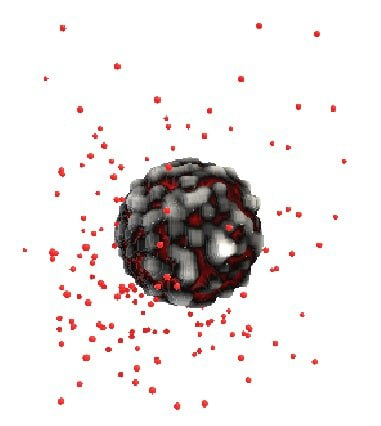
\includegraphics[scale=0.7]{img/no_inm.jpg}
\caption{Imagen tomada de simulaci\'on de tumor sin tener en cuenta la intervenci\'on de c\'elulas inmunol\'ogicas. Los puntos rojos son las c\'elulas migratorias que salen desde el tumor principal. Generaci\'on n\'umero 46, radio del tumor 22.81.}
\end{figure}

\begin{figure}[htb]
\centering
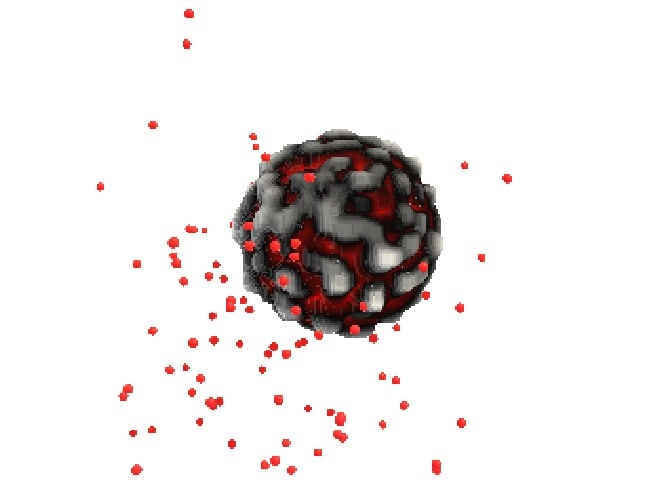
\includegraphics[scale=0.7]{img/inm.jpg}
\caption{Imagen tomada de simulaci\'on de tumor teniendo en cuenta la intervenci\'on de c\'elulas inmunol\'ogicas. Los puntos rojos son las c\'elulas migratorias que salen desde el tumor principal. Generaci\'on n\'umero 46, radio del tumor 20.67.}
\end{figure}


Se obtuvo una representaci\'on del proceso de aparici\'on, evoluci\'on y desaparici\'on de las micromet\'astasis. Se puede apreciar como a partir de generaciones avanzadas, estos pequeños tumores van apareciendo.\\

\begin{figure}[htb]
\centering
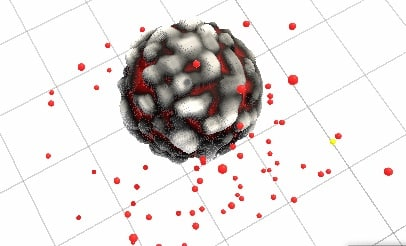
\includegraphics[scale=0.7]{img/met.jpg}
\caption{Puntos amarillos, c\'elulas de micromet\'astasis. Esta imagen representa las c\'elulas migratorias que lograron hacer micromet\'astasis en un tumor secundario, donde muchas de ella son eliminadas  debido al sistema inmune o que no se logran adaptar al nuevo ambiente del \'organo secundario que es diferente a las condiciones que exist\'ian en el \'organo origen donde surgieron.}
\end{figure}


\newpage
\section{\bf{Conclusiones}}
En el presente trabajo se desarroll\'o un aut\'omata que modela el ciclo de vida del c\'ancer en el tejido epitelial, especif\'icamente para el c\'ancer de mama.Para el desarrollo de este se defini\'o un conjunto de c\'elulas y la funci\'on de vecindad del aut\'omata mediante una red de mundo peque\~no utilizando el modelo de Watts-Strogatz. Se cre\'o un conjunto de estados para las c\'elulas del aut\'omata que representa diversas poblaciones celulares entre estas que se encuentran las c\'elulas normales , cancer\'igenas e inmunes. Se defini\'o una funci\'on de transici\'on y su actualizaci\'on , que describen satisfactoriamente el desarrollo tumoral avascular y vascular. Se obtuvieron resultados visuales en 3D de todos los procesos representados por el aut\'omata celular evidenciando el comportamiento realista del mismo mediante la comparaci\'on con los resultados experimentales existentes en la literatura.\\



A modo de conclusi\'on se puede decir que este trabajo alcanz\'o su objetivo puesto que se logr\'o llevar el trabajo realizado por Darien \cite{1} a un plano 3d y se incluyen las c\'elulas inmunes que no eran tenidas en cuenta en el \'organo principal.

\newpage
\section{\bf{Recomendaciones}}
Para la ampliaci\'on y perfeccionamiento de este trabajo se mencionan una serie de recomendaciones acontinuaci\'on:
\begin{itemize}
\item Ampliar el modelo para que incorpore mecanismos que permitan reproducir el recrecimiento tumoral cuando se lleva a cabo tratamientos quir\'urgicos o terapias dirigidas a disminuir el tama\~no del tumor para su estudio.
\item Se propone desarrollar un modelo que permita obtener crecimientos, migraciones y
capacidades metast\'asicas variables para cada neoplasia, puesto que en el presente las neoplasias de una misma simulac\'on poseen los mismos par\'ametros por lo que el comportamiento es similar.

\end{itemize}

\begin{thebibliography}{99}

\bibitem{1} Darien Viera Barredo. Tesis de diploma defendida en Departamento de Matem\'atica, Facultad de Matem\'atica y Computaci\'on.  Universidad de La Habana, June, 2019. 
\bibitem{inmunidad} Huricha Ruanxiaogang.A Simple Cellular Automaton Model for Tumor-immunity System.Beijing Polytechnic University School of Electronic Information and Control Engineering Beijing.

\bibitem{2} R. Albert and A. L\'aszl\' Barab\'asi. Statistical mechanics of complex networks. Reviews of
modern physics, 74, 2002.

\bibitem{3} Duncan J. Watts and Steven H. Strogatz. Collective dynamics of small-world networks.
Nature, 393:440–442, 1998.
	
\bibitem{wiki} Wikipedia. URL: \href{http://en.wikipedia.org}{http://en.wikipedia.org}.
Consultado en \today.

\end{thebibliography}
\smallskip
\smallskip

\end{document}